\part{Contribution}

\chapter{Privilege Flow Graphs for Detecting Access Control 
Vulnerabilities via Graph Neural Networks}
\label{ch:detection}

% =====================================================================
\section{Introduction}
\label{det:intro}
% =====================================================================

Authorization vulnerabilities occupy a peculiar position in the landscape of
software security flaws. Unlike injection attacks, which leave a syntactic
fingerprint wherever tainted data meets an interpreter, or memory corruption,
which arises from a violation of type safety that a compiler can in principle
catch, authorization flaws are defined by what the program \emph{does not
do}. A missing decorator, an absent filter clause, a forgotten role check
before a privileged mutation. Each is a structural gap in the security
architecture rather than a localized code defect. The danger is not in what
the developer wrote, but in what they neglected to write.

This observation has a direct methodological consequence. Detection
techniques built to recognise the \emph{presence} of dangerous patterns
(taint propagation from a user-controlled source to a sensitive sink,
unsafe memory operations, suspicious API sequences) are fundamentally
ill-suited to a problem defined by \emph{absence}. A token-level model
cannot learn what is not there. A taint analyser cannot trace a flow that
does not exist. A pattern matcher has no pattern to match. Authorization
vulnerabilities therefore call for a representation and a reasoning mode
that are qualitatively different from those the community has developed for
injection, XSS, or buffer overflow.

This chapter develops the \emph{Privilege Flow Graph} (PFG), a domain-specific
graph formalism designed to make the authorization architecture of a web
application explicit, inspectable, and amenable to both formal reasoning and
learned classification. The PFG is not a general-purpose code
representation. It does not model control flow, data flow, or syntactic
structure in the usual sense. It captures precisely the four kinds of
components that participate in authorization decisions (entry points,
protective guards, intermediate logic, and terminal data operations) and the
three kinds of relationships that connect them. On this deliberately narrow
representation, we develop a hybrid detection architecture that combines the
generalization capacity of graph neural networks with the precision and
interpretability of structural rules expressed as first-order logic
predicates.


% =====================================================================
\section{Problem Formulation}
\label{det:problem}
% =====================================================================

Before a detection claim can be evaluated, the problem it addresses must be
fixed without ambiguity. This section does that work. We define the threat
model, develop the vulnerability taxonomy that structures the detection
target, diagnose the three structural gaps in existing detection approaches,
and crystallise the analysis into testable hypotheses. The vocabulary
introduced here is reused throughout the chapter; it forms the contract
between the formalism and the implementation.

\subsection{Attacker model and security scope}
\label{sec:det-threat}
\textcolor{red}{}

We fix a web application $\mathcal{A}$ exposing a set of REST API endpoints
over HTTP. The application comprises a routing layer that maps incoming
requests to handler functions, a middleware layer that may interpose
protective checks (authentication, authorization) before the handler
executes, a service layer containing business logic, and a data access layer
that issues database operations. This layered model is not an idealisation;
it is the explicit architectural pattern enforced by every major REST
framework, including Django, Spring Boot, Flask, Express, ASP.NET, and
FastAPI, differing only in the syntactic mechanisms (decorators, annotations,
filter chains, dependency injection) through which each layer is configured.

\texttt{Attacker profile:} the adversary is an authenticated user in
possession of valid credentials who attempts horizontal or vertical privilege
escalation. Horizontal escalation targets resources belonging to other users
at the same privilege level; vertical escalation targets administrative
operations requiring elevated privileges. We exclude unauthenticated attack
scenarios (handled by perimeter security) and injection-based attacks
(handled by input validation). This scoping is deliberate: the attacker we
model is precisely the one that traditional SAST tools cannot see, because
the attack vector is not a malicious input but a \emph{legitimate request
to the wrong endpoint}.

\texttt{Protected assets:} the protected assets are the data objects
accessed by terminal database operations. Each endpoint ultimately reads,
creates, modifies, or deletes resources through one or more data access
operations. The security requirement is that every such operation be
reachable only by users with sufficient authorization for the specific
resource being accessed.

\texttt{Trust boundary:} the authorization decision chain follows a
three-stage model:
\begin{enumerate}
    \item \textit{Authentication}: verification that the requesting entity
    possesses a valid identity (session token, JWT, API key).
    \item \textit{Authorization}: enforcement of access control policies
    restricting which authenticated identities may access which resources
    under which conditions.
    \item \textit{Data access}: the terminal database operation that reads,
    creates, modifies, or deletes a resource.
\end{enumerate}

\begin{figure}[htbp]
\centering
\includegraphics[width=1\linewidth]{figures/fig_threat_model.png}
\caption{Threat model overview.}
\label{fig:det-threat-model}
\end{figure}

A vulnerability exists when the authorization stage is absent or
insufficient relative to the sensitivity of the data access operation it
precedes. The trust boundary lies between authentication and data access;
the goal is to detect gaps in this boundary.

%\paragraph{Scope and framework independence.}
The PFG formalism targets any web framework that implements REST endpoints
with middleware-based authorization. The abstraction requires only that the
framework expose (statically or through well-defined patterns) three kinds
of information: which routes exist, what guards protect them, and what data
operations they perform. We instantiate and evaluate concrete extractors for
two representative frameworks: Django REST Framework (DRF), representing the
Python ecosystem, and Spring Boot, representing the Java ecosystem. The
formalism itself makes no assumption specific to either. A Flask application
with \texttt{@login\_required} decorators, or an Express application with
\texttt{passport} middleware, would yield a structurally identical PFG given
an appropriate extractor. This point is not incidental; it is the foundation
of the generality claim.

\subsection{Taxonomy of authorization vulnerabilities}
\label{sec:det-taxonomy}

Broken Access Control (A01:2021) holds the number one position in the OWASP
Top~10 (2021 edition), the most critical web application security risk,
elevated from fifth place in 2017 based on incidence data from over 400,000
applications. Building on this classification and the Common Weakness
Enumeration, we identify five structurally distinct subtypes of authorization
vulnerabilities that the PFG is designed to detect. Each represents a
different failure mode in the authorization decision chain, and each has a
distinct structural signature in the graph.

\begin{itemize}

\item \texttt{MISSING\_AUTH (CWE-306):}
An endpoint performs data access without requiring any form of
authentication, allowing anonymous users to invoke the operation and access
the underlying data. Formally, an endpoint $v$ exhibits this vulnerability
if and only if $v$ requires no authentication, $v$ reaches at least one data
access node via call edges, and $v$ is not designated as intentionally public.

\item \texttt{MISSING\_ROLE (CWE-862):}
An authenticated endpoint performs a privileged mutation (write, update,
delete on shared resources) without verifying that the requesting user holds
the requisite privilege level. An endpoint $v$ exhibits this vulnerability
if $v$ requires authentication, $v$ reaches a data access performing a
privileged operation on a shared entity, and no node on any call path from
$v$ to the data access enforces a role check.

\item \texttt{IDOR: Insecure Direct Object Reference (CWE-639):}
An endpoint accepts a user-controlled identifier (route parameter) that
flows to a database query without verifying that the authenticated user owns
or has permission to access the referenced object. An endpoint $v$ exhibits
this vulnerability if $v$ contains route parameters, an identifier flow edge
connects $v$ to a data access node $d$, the data access targets an
ownership-bearing entity, no node on any call path from $v$ to $d$ enforces
an ownership check, and $d$ has no ownership predicate in its query filter.

\item \texttt{TENANT\_ISOLATION\_FAILURE:}
In multi-tenant applications, a data access retrieves resources across
tenant boundaries without enforcing tenant-scoped filtering. An endpoint $v$
exhibits this vulnerability if $v$ reaches a data access node $d$ whose
target entity requires tenant isolation, $d$ has no tenant predicate in its
query filter, and no middleware on the path from $v$ to $d$ enforces tenant
scoping.

\item \texttt{OBJECT\_LEVEL\_PERMISSION\_BYPASS:}
An endpoint has evidence of model-level permissions (the application defines
object-level access control for the resource) but the specific endpoint does
not enforce object-level authorization when accessing individual objects via
route parameters. An endpoint $v$ exhibits this vulnerability if $v$ has
model-level permission indicators, $v$ accepts route parameters and reaches a
data access via identifier flow, and no object-level permission check is
enforced on any call path to the data access.

\end{itemize}

\subsection{Gaps in existing detection approaches}
\label{sec:det-gaps}

We identify three structural gaps that explain why existing detection
paradigms fail on authorization vulnerabilities. Each gap maps directly to a
design choice in the PFG framework.

\begin{enumerate}

\item \textbf{Representation granularity mismatch:}
Code Property Graphs (CPGs) \citep{yamaguchi2014modeling} and similar
statement-level representations model every syntactic element, control flow
edge, and data dependency at the instruction level. For a typical 20-line
view handler, the CPG contains several hundred nodes. Yet the
authorization-relevant information can be expressed in 3--5 nodes: one entry
point, zero or more guards, and one or more data operations. The signal
(``does a sufficient guard exist between this endpoint and this database
query'') is buried under structure that is irrelevant to the problem.
Constructing a CPG for a full application (500+ endpoints) produces graphs
with millions of nodes; GNN inference over such structures is prohibitive
and yields diminishing returns because the vast majority of the topology has
nothing to do with authorization.

\item \textbf{Token-window blindness:}
Pre-trained language models for code (CodeBERT \citep{feng2020codebert},
VulBERTa \citep{hanif2022vulberta}, LineVul \citep{fu2022linevul}) encode
source in fixed-length token windows, typically 512 tokens
\citep{feng2020codebert}. An authorization decision involves at minimum three
files (the URL configuration, the view handler, and the data model) and the
security-critical relationship between them cannot fit in a single window.
More fundamentally, these models learn to detect the \emph{presence} of
vulnerability-indicative patterns, but authorization flaws are defined by
what is \emph{missing}: a decorator that should be there, a filter clause
that should constrain a queryset. Learning the absence of a pattern is
inherently harder than learning its presence, and no amount of pre-training
resolves the gap when the window cannot even hold all the relevant files.

\item \textbf{No structural explanation:}
Pattern-based SAST tools (Semgrep, CodeQL) express rules over local code
patterns. They can match the presence of a dangerous call but cannot reason
about the absence of a required guard on a cross-component path. When they
fire (which is rare for authorization), the explanation is a pattern match,
not a structural path through the application architecture. Security
engineers need to know \emph{which} endpoint, \emph{which} data access,
and \emph{which} guard is missing. This information can only be provided
by a structural representation.
  
\end{enumerate}


\subsection{Hypotheses}
\label{sec:det-hypotheses}

The analysis above yields three hypotheses that the rest of the chapter
tests:
\begin{itemize}%[leftmargin=1.8em,style=nextline]
  \item \textbf {H1:}
  A graph representation that captures only authorization-relevant
  components (endpoints, guards, services, data accesses) and their
  relationships is sufficient to detect authorization vulnerabilities that
  are invisible to general-purpose representations.

  \item \textbf {H2:}
  A graph neural network trained on structural patterns of vulnerable and
  safe authorization architectures can learn to classify endpoints, even
  though the vulnerability signal is the absence of protective structure
  rather than the presence of dangerous patterns.

  \item \textbf {H3:}
  Combining a neural scorer (for generalization) with a logical validator
  (for precision and explanation) yields better detection performance than
  either in isolation, and provides interpretable explanations without
  requiring post-hoc explainability tools.
\end{itemize}

\subsection{Research questions}
\label{sec:det-rqs}

We operationalise the hypotheses into three testable research questions:
\begin{enumerate}
    \item \textbf{RQ1:}
    Can a domain-specific graph representation effectively detect access
    control vulnerabilities in production web applications?
    \item \textbf{RQ2:}
    Does the framework provide interpretable, actionable results without
    requiring post-hoc explanation techniques?
    \item \textbf{RQ3:}
    How does hybrid PFG-based detection compare with rule-based structural
    analysis and existing static analysis tools?
\end{enumerate}


% =====================================================================
\section{Proposed Approach and Architecture}
\label{det:design}
% =====================================================================

Having fixed the problem, we can now describe the solution. This section
develops the PFG formalism and the hybrid detection architecture that
operates on it. The presentation is top-down: we begin with the
architectural intuition that motivates the design, formalise the graph
structure, justify the feature space, develop the neural and logical
detection components, and close with the complementarity argument. All
implementation detail (extraction algorithms, training methodology, corpus
construction) is deferred to Section~\ref{det:impl}; here the concern is
the \emph{what} and the \emph{why}, not the \emph{how}.

\begin{figure}[ht]
\centering
\includegraphics[width=0.85\linewidth]{figures/fig_det_overview.png}
\caption{End-to-end overview of the PFG-based detection approach.}
\label{fig:det-overview}
\end{figure}

\subsection{Design rationale}
\label{sec:det-intuition}

Before the formalism, consider the intuition. Any REST API, regardless of
implementation language or framework, has a common structural backbone when
viewed through the lens of authorization: requests arrive at \emph{entry
points} (routes, endpoints), pass through zero or more \emph{protective
guards} (authentication checks, role verifications, ownership validations),
flow through \emph{service logic} (business computations, nested calls), and
terminate at \emph{data operations} (database reads, writes, updates,
deletes). A vulnerability exists when the chain of guards between an entry
point and a data operation is insufficient for the sensitivity of that
operation.

This observation suggests a representation strategy: discard everything in
the application that is not one of these four components or one of the
relationships between them. The resulting graph will be small (a few dozen
nodes versus the hundreds of thousands in a CPG), every element will have a
direct security interpretation, and the vulnerability question becomes a
structural property of paths in the graph. This is the Privilege Flow Graph.

The PFG deliberately sacrifices generality for focus. It cannot represent
arbitrary security properties; it cannot model injection, XSS, or race
conditions. What it \emph{can} do is represent the authorization
architecture of any REST API with a precision and compactness that no
general-purpose representation matches. The sacrifice is calculated: we
trade broad applicability for deep effectiveness on a single, important, and
underserved problem class.

\subsection{Formal graph definition}
\label{sec:det-pfg-def}

\begin{definition}[Privilege Flow Graph]
\label{def:pfg}
A Privilege Flow Graph is a directed, typed, attributed graph defined as the
6-tuple:
\begin{equation}
G = (V, E, \tau_V, \tau_E, \phi_V, \phi_E)
\end{equation}
where:
\begin{itemize}
    \item $V$ is the finite set of nodes,
    \item $E \subseteq V \times V$ is the set of directed edges,
    \item $\tau_V: V \to \{\textsc{endpoint}, \textsc{middleware},
    \textsc{service}, \textsc{data\_access}\}$ assigns each node its type,
    \item $\tau_E: E \to \{\textsc{call}, \textsc{identifier\_flow},
    \textsc{tenant\_flow}\}$ assigns each edge its type,
    \item $\phi_V: V \to \mathbb{R}^{36}$ maps each node to its feature
    vector,
    \item $\phi_E: E \to \mathbb{R}^{3}$ maps each edge to its feature
    vector (one-hot encoding of edge type).
\end{itemize}
\end{definition}

The PFG schema is specified as a JSON Schema (version 1.0, shipped in
\texttt{schemas/pfg-1.0.json}) and all generated graphs are validated
against this schema at construction time. Structural consistency is enforced
rather than assumed.

\subsection{Node types and their semantic role}
\label{sec:det-nodes}

Each node type corresponds to a specific role in the authorization decision
chain. Together, they partition the application's security-relevant
architecture into four orthogonal concerns. Their definition is
framework-independent: any REST framework that exposes routes, guards, and
data operations admits an instantiation.


\begin{itemize}

\item \texttt{ENDPOINT nodes: } An \textsc{endpoint} node represents the entry point where an HTTP request
enters the application. It encodes the route pattern, accepted HTTP methods,
route parameters, and initial authorization signals derived from the
framework's configuration. The endpoint is the origin of all authorization
reasoning: \emph{what protections should this entry point carry, given what
data it ultimately accesses?}

In Django, an endpoint corresponds to a view function or class method
registered in the URL configuration. In Spring Boot, it corresponds to a
controller method annotated with a request-mapping annotation. In Flask, it
would correspond to a route-decorated function. The PFG abstraction unifies
all three into a single node type with identical attributes.


\item \texttt{MIDDLEWARE nodes:} A \textsc{middleware} node represents a protective guard interposed between
the entry point and the data access. Each middleware has a guard type drawn
from five categories: \textsc{authentication} (verifies identity),
\textsc{role\_check} (verifies privilege level),
\textsc{ownership\_check} (verifies resource ownership),
\textsc{tenant\_check} (enforces tenant boundaries), and
\textsc{object\_permission\_check} (enforces fine-grained object-level
permissions).

The presence or absence of middleware nodes on paths from endpoints to data
access nodes constitutes the primary vulnerability signal in the PFG. A
missing middleware \emph{is} the vulnerability; the representation makes
this absence structurally visible rather than requiring inference from what
the code does not say.

\item \texttt{SERVICE nodes:} A \textsc{service} node represents intermediate business logic invoked along
the call chain between an endpoint and its data access operations. Service
nodes model functional layers (business services, utility functions, nested
view calls) and serve as routing vertices in the call graph. While not
directly involved in authorization decisions, they enable accurate path
reconstruction for vulnerability explanation.

\item \texttt{DATA\_ACCESS nodes:} A \textsc{data\_access} node represents a terminal database operation. Its
attributes encode the operation type (\textsc{read}, \textsc{write},
\textsc{update}, \textsc{delete}), the target entity (database model),
ownership predicates (whether the query filters by requesting user), tenant
predicates (whether the query scopes to the requesting tenant), and
object-permission indicators.

\end{itemize}

%\paragraph{Vulnerability as a path property.}
With these four types defined, the central insight can be stated precisely:
\begin{quote}
\emph{An authorization vulnerability exists when a path from an
\textsc{endpoint} to a \textsc{data\_access} node lacks sufficient
\textsc{middleware} given the sensitivity of the data access operation at
the terminus.}
\end{quote}
This is not a heuristic or an approximation. It is the formal definition of
the detection target, and the five vulnerability subtypes above are simply
specialisations of what ``sufficient middleware'' means for different
combinations of endpoint properties and data access characteristics.



\subsection{Edge types}
\label{sec:det-edges}

Three edge types capture the relationships between nodes:
\begin{itemize}
    \item \texttt{CALL} ($\tau_E = \textsc{call}$): function invocation,
    connecting endpoints to services, services to other services, and
    services to data access nodes. These edges form the call graph backbone.

    \item \texttt{IDENTIFIER\_FLOW} ($\tau_E = \textsc{identifier\_flow}$):
    tracks how user-controlled identifiers (route parameters) propagate from
    endpoints to data access operations. The presence of an identifier flow
    edge from an endpoint to a data access node is a necessary condition for
    IDOR.

    \item \texttt{TENANT\_FLOW} ($\tau_E = \textsc{tenant\_flow}$): tracks
    tenant-scoping information flow from authentication context to data
    access queries. Their absence on paths to tenant-sensitive data indicates
    a potential tenant isolation failure.
\end{itemize}

\begin{figure}[htbp]
\centering
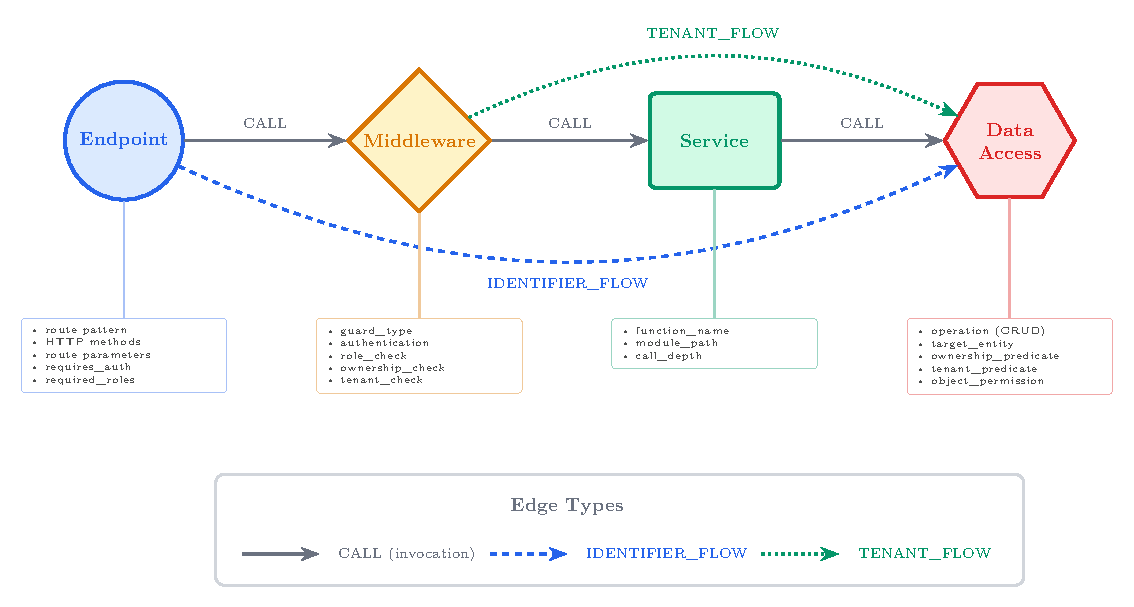
\includegraphics[width=\linewidth]{figures/fig_pfg_schema.pdf}
\caption{PFG graph schema: node types, edge types, and attributes.}
\label{fig:det-schema}
\end{figure}

\subsection{Feature space}
\label{sec:det-features}

The node feature function $\phi_V: V \to \mathbb{R}^{36}$ encodes each node
as a 36-dimensional vector. Unlike learned embeddings in NLP approaches,
every dimension corresponds to a human-interpretable security property. This
design choice ensures the feature space is fully transparent and auditable
, a property we regard as non-negotiable for security tooling.

Table~\ref{tab:det-features} provides the specification. The vector is
structured in layers of increasing specificity:
\begin{itemize}
    \item \texttt{Structural identity} (indices 0--8): node type (one-hot,
    4 bits) and HTTP method (one-hot, 5 bits) establish the node's role and
    risk profile.
    \item \texttt{Direct authorization signals} (indices 9--15): properties
    read from framework configuration indicating whether an authorization
    mechanism is present.
    \item \texttt{Guard evidence} (indices 16--18): for middleware nodes, the
    type of protection they provide.
    \item \texttt{Data access characterization} (indices 19--23): the nature
    and sensitivity of the terminal operation.
    \item \texttt{Structural reachability} (indices 24--35): computed
    features encoding relationships between the node and its graph
    neighborhood, specifically whether unprotected data is reachable, whether identifier
    flows exist without corresponding guards.
\end{itemize}

\begin{table}[htbp]
\centering
\caption{PFG node feature vector specification ($\phi_V \in \mathbb{R}^{36}$).
Every dimension is a named, interpretable security property.}
\label{tab:det-features}
\small
\begin{tabular}{@{}clll@{}}
\toprule
\textbf{Idx} & \textbf{Property} & \textbf{Encoding} & \textbf{Detection Role} \\
\midrule
$[0{:}4]$ & Node type & One-hot & Graph structure \\
$[4{:}9]$ & HTTP method & One-hot & Risk profile \\
$[9]$ & \texttt{requires\_auth} & Binary & MISSING\_AUTH \\
$[10{:}15]$ & Required role & One-hot & MISSING\_ROLE \\
$[15]$ & Ownership check & Binary & IDOR \\
$[16{:}19]$ & Guard type & One-hot & Path protection \\
$[19{:}23]$ & Operation type & One-hot & Damage potential \\
$[23]$ & Ownership predicate & Binary & IDOR (data-level) \\
$[24]$ & Has route params & Binary & IDOR prerequisite \\
$[25]$ & Reachable data count & Normalized & Exposure scope \\
$[26]$ & Has identifier flow & Binary & IDOR prerequisite \\
$[27]$ & Unprotected data & Binary & Multi-subtype \\
$[28]$ & Role check present & Binary & MISSING\_ROLE \\
$[29]$ & Model permission & Binary & OBJ\_PERM\_BYPASS \\
$[30]$ & Object permission & Binary & OBJ\_PERM\_BYPASS \\
$[31]$ & Tenant check & Binary & TENANT\_ISO \\
$[32]$ & Has tenant scope & Binary & TENANT\_ISO \\
$[33]$ & Unscoped tenant data & Binary & TENANT\_ISO \\
$[34]$ & Obj-perm data reach & Binary & OBJ\_PERM\_BYPASS \\
$[35]$ & Tenant/obj signal & Continuous & Multi-subtype \\
\bottomrule
\end{tabular}
\end{table}

%\paragraph{Feature values for non-ENDPOINT nodes.}
Indices 9--15 and 24--26 are primarily meaningful for \textsc{endpoint}
nodes. For \textsc{middleware} nodes, indices 16--18 carry the guard type
while endpoint-specific indices are zeroed. For \textsc{data\_access} nodes,
indices 19--23 carry the operation type, and indices 23, 31--33 carry
predicate information. \textsc{service} nodes receive only the node type
encoding at indices 0--3; all other positions are zero. This sparse encoding
is intentional: the GNN learns to propagate relevant information across
edges rather than requiring each node to carry a complete summary.

%\paragraph{On transparency.}
The critical property of this feature space is that every dimension admits a
human-readable explanation. A developer inspecting a prediction can identify
immediately which features contribute: ``this endpoint has
\texttt{requires\_auth=0}, \texttt{reachable\_data\_count=3}, and
\texttt{ownership\_check=0}.'' No opaque embedding, no hidden activation to
decode. This property is deliberate, and it is what underwrites the
interpretability claim of contribution D2.

\subsection{GATv2-based classification}
\label{sec:det-gnn}

We select Graph Attention Network v2 (GATv2) \citep{brody2021attentive} as
the message-passing backbone for the neural component. The choice is
motivated by the asymmetric nature of authorization relationships in the
PFG: the protective effect of a middleware node on an endpoint depends on
\emph{which} data access the endpoint reaches, and the severity of an
unprotected path depends on the sensitivity of the terminal operation.
Static attention (as in the original GAT \citep{velivckovic2018graph}) cannot
capture this context dependence; GATv2's dynamic attention computes
relevance as a function of both source and target node features, which is
precisely what the problem requires.

%\subsubsection{Message-passing equations}

Given node features $\mathbf{h}_i^{(l)} \in \mathbb{R}^d$ at layer $l$ and
edge features $\mathbf{e}_{ij} \in \mathbb{R}^3$, the GATv2 layer computes
updated representations through the following attention mechanism. We
incorporate edge features into the attention computation following the PyG
\texttt{GATv2Conv(edge\_dim=...)} variant, extending the base formulation
of Brody et al.\ \citep{brody2021attentive} to condition attention on edge
type:
\begin{equation}
\label{eq:det-gatv2}
\alpha_{ij}^{(l)} = \frac{
  \exp\!\left(\mathbf{a}^{\top}
  \mathrm{LeakyReLU}\!\left(\mathbf{W}\left[
  \mathbf{h}_i^{(l)} \| \mathbf{h}_j^{(l)} \| \mathbf{e}_{ij}
  \right]\right)\right)
}{
  \sum_{k \in \mathcal{N}(i)} \exp\!\left(\mathbf{a}^{\top}
  \mathrm{LeakyReLU}\!\left(\mathbf{W}\left[
  \mathbf{h}_i^{(l)} \| \mathbf{h}_k^{(l)} \| \mathbf{e}_{ik}
  \right]\right)\right)
}
\end{equation}
where $\mathbf{W} \in \mathbb{R}^{d' \times (2d + 3)}$ is the shared weight
matrix, $\mathbf{a} \in \mathbb{R}^{d'}$ is the attention vector, $\|$
denotes concatenation, and $\mathcal{N}(i)$ is the neighborhood of node $i$.
The updated representation aggregates neighbor information weighted by the
computed attention:
\begin{equation}
\label{eq:det-update}
\mathbf{h}_i^{(l+1)} = \Big\|_{k=1}^{K} \sum_{j \in \mathcal{N}(i)}
\alpha_{ij}^{(l,k)} \mathbf{W}^{(k)} \mathbf{h}_j^{(l)}
\end{equation}
where $K$ is the number of heads and $\|$ denotes head concatenation.

%\paragraph{Why attention matters here.}
Consider a middleware node $m$ of type \textsc{ownership\_check} on a path
between endpoint $v$ and data access $d$. The relevance of $m$ to the
vulnerability classification of $v$ depends on whether $d$ is an
ownership-bearing entity (if not, the ownership check is irrelevant),
whether the identifier flow actually passes through $m$ (if it bypasses the
guard, no protection is conferred), and whether other guards on the same
path provide equivalent protection. Dynamic attention allows the model to
learn these context-dependent relevance weights rather than treating all
neighbors as equally important.

\subsection{Target-aware attention pooling}
\label{sec:det-pooling}

After $L$ layers of message passing, each node $i$ carries a contextualised
representation $\mathbf{h}_i^{(L)} \in \mathbb{R}^{d}$ encoding both its own
features and propagated neighborhood information. To classify a specific
endpoint, we must aggregate the graph into a fixed-size representation while
maintaining focus on the target node.

Standard global pooling (mean, max, sum) loses target-specificity: the same
pooled vector would be produced regardless of which endpoint is being
evaluated. This is inadequate because a single application graph may contain
multiple endpoints that are simultaneously safe at some nodes and vulnerable
at others. We introduce a target-aware mechanism:

\begin{equation}
\label{eq:det-score}
s_i = \mathbf{w}^{\top} \tanh\!\left(\mathbf{W}_s \left[\mathbf{h}_i \|
\mathbf{h}_{\mathrm{target}}\right]\right)
\end{equation}
\begin{equation}
\label{eq:det-alpha}
\alpha_i = \frac{\exp(s_i)}{\sum_{j \in V} \exp(s_j)}
\end{equation}
\begin{equation}
\label{eq:det-pool}
\mathbf{z} = \sum_{i \in V} \alpha_i \, \mathbf{h}_i
\end{equation}
\begin{equation}
\label{eq:det-class}
\hat{y} = \mathrm{MLP}\!\left(\left[\mathbf{z} \|
\mathbf{h}_{\mathrm{target}}\right]\right)
\end{equation}
where $\mathbf{h}_{\mathrm{target}}$ is the representation of the endpoint
being classified (the node whose vulnerability status we are predicting),
$\mathbf{W}_s \in \mathbb{R}^{d \times 2d}$ and $\mathbf{w} \in
\mathbb{R}^{d}$ are learnable parameters, and the final MLP maps from
$\mathbb{R}^{2d}$ to $\mathbb{R}^{C}$ where $C = 8$ is the number of
classes.

The attention score $s_i$ measures how relevant each node $i$ is to the
classification of the target endpoint. Nodes structurally important to the
target's security posture (its guards, its data access operations,
intermediate services on its paths) receive higher weights, while nodes
belonging to other subgraphs are down-weighted. The mechanism ensures the
model's classification focuses on the local security context of the specific
endpoint under evaluation.

%\paragraph{Output classes.}
The classifier produces scores over 8 classes: \textsc{safe},
\textsc{missing\_auth}, \textsc{missing\_role}, \textsc{idor},
\textsc{tenant\_isolation\_failure},
\textsc{object\_level\_permission\_bypass}, \textsc{combined}, and
\textsc{intentionally\_public}. The \textsc{combined} class handles
endpoints exhibiting multiple simultaneous vulnerabilities (e.g., both IDOR
and missing role); the \textsc{intentionally\_public} class distinguishes
endpoints that are deliberately unauthenticated (login, registration, health
checks) from those that are accidentally so.

\begin{figure}[htbp]
\centering
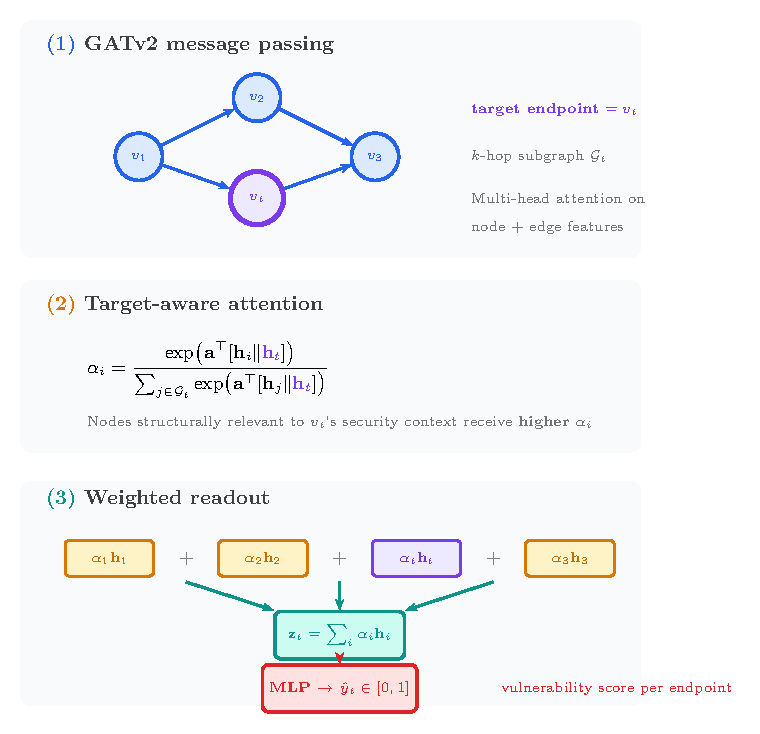
\includegraphics[width=0.85\linewidth]{figures/fig_pooling.pdf}
\caption{Target-aware attention pooling mechanism. (1)~GATv2 message passing produces contextualised node representations over the $k$-hop subgraph around target endpoint $v_t$. (2)~Attention scores $\alpha_i$ are computed relative to the target's representation, weighting nodes by their structural relevance to $v_t$'s security context. (3)~Weighted readout produces a fixed-size graph embedding $\mathbf{z}_t$ that is concatenated with $\mathbf{h}_t$ and passed to the classification MLP.}
\label{fig:det-pooling}
\end{figure}

\subsection{Structural rules as formal predicates}
\label{sec:det-rules}

The rule-based component provides guaranteed interpretability and serves
both as a standalone baseline and as a validation layer for GNN predictions.
Each rule is formalized as a predicate over endpoints in the PFG: given an
endpoint $v$, the predicate evaluates to true when the structural conditions
for a specific vulnerability subtype are satisfied.

\begin{definition}[Rule $R_1$: Missing Authentication]
\begin{equation}
R_1(v): \tau_V(v) = \textsc{ep} \wedge \neg\mathrm{auth}(v) \wedge
\mathrm{reaches\_da}(v) \wedge \neg\mathrm{public}(v) \implies
\textsc{missing\_auth}(v)
\end{equation}
\end{definition}

\begin{definition}[Rule $R_2$: Missing Role Check]
\begin{equation}
R_2(v): \mathrm{auth}(v) \wedge \mathrm{reaches\_priv}(v) \wedge
\neg\exists\, m \in \mathrm{path}(v,d) : \mathrm{guard}(m) = \textsc{role}
\implies \textsc{missing\_role}(v)
\end{equation}
\end{definition}

\begin{definition}[Rule $R_3$: IDOR]
\begin{equation}
R_3(v): \mathrm{has\_param}(v) \wedge \exists\,(v,d) \in
E_{\textsc{id\_flow}} \wedge \neg\mathrm{own\_on\_path}(v,d) \implies
\textsc{idor}(v)
\end{equation}
\end{definition}

\begin{definition}[Rule $R_4$: Tenant Isolation Failure]
\begin{equation}
R_4(v): \mathrm{reaches\_tenant\_data}(v) \wedge
\neg\mathrm{tenant\_scoped}(v,d) \implies \textsc{tenant\_iso}(v)
\end{equation}
\end{definition}

\begin{definition}[Rule $R_5$: Object-Level Permission Bypass]
\begin{equation}
R_5(v): \mathrm{model\_perm}(v) \wedge \mathrm{has\_param}(v) \wedge
\neg\mathrm{obj\_perm\_on\_path}(v,d) \implies \textsc{obj\_perm\_bypass}(v)
\end{equation}
\end{definition}

The auxiliary predicates are defined as:
\begin{itemize}
    \item $\mathrm{reaches\_da}(v)$: $\exists\, d \in V$ with $\tau_V(d) =
    \textsc{data\_access}$, reachable from $v$ via call edges,
    \item $\mathrm{reaches\_priv}(v)$: $v$ reaches a data access performing
    WRITE, UPDATE, or DELETE,
    \item $\mathrm{path}(v,d)$: all simple paths from $v$ to $d$ via call
    edges, bounded by a configurable depth limit (default 8, a parameter
    chosen to cover the deepest call chains observed in the evaluation
    corpus without incurring combinatorial explosion on recursive
    structures),
    \item $\mathrm{own\_on\_path}(v,d)$: $\exists\, m \in \mathrm{path}(v,d)$
    that is an ownership guard, or $d$ has an ownership predicate,
    \item $\mathrm{tenant\_scoped}(v,d)$: tenant check on path or tenant
    predicate at $d$.
\end{itemize}

%\paragraph{Soundness within the formalization.}
The rules are sound relative to the threat model: if the structural
conditions of $R_i(v)$ are satisfied and the PFG is correctly constructed,
then endpoint $v$ is vulnerable by the definitions of
Section~\ref{sec:det-taxonomy}. This guarantee is, however, conditioned on
two assumptions that may fail in practice: (1)~the extractor correctly
identifies all relevant guards (a guard missed by the extractor will cause a
false positive), and (2)~the threat model captures all relevant protection
mechanisms (an application-specific guard pattern not modeled in the PFG will
likewise cause a false positive). We return to the empirical consequences
of these assumptions in Section~\ref{det:discussion}.

\subsection{Complementarity of neural and logical components}
\label{sec:det-complement}

The two components serve distinct roles:
\begin{itemize}
    \item \textbf{Rules, precision and interpretability}: Every rule
    firing produces a concrete explanation grounded in the specific nodes and
    edges involved. The explanation IS the detection mechanism: ``Route
    parameter \texttt{id} of \texttt{PUT /api/v2/workout/\{id\}/} reaches
    UPDATE on \texttt{Workout} via 1 call path; none enforce ownership.
    Subtype: IDOR.'' No post-hoc technique is needed.

    \item \textbf{GNN, selectivity and generalization}: The neural
    component captures interaction effects that exceed the expressiveness of
    boolean predicates. For instance, it may learn that certain combinations
    of features across a multi-hop neighborhood indicate safety even when
    individual rule conditions are met, such as a service node implementing
    a custom permission check not explicitly modeled as a middleware.
    The GNN's primary role is to suppress false positives by providing
    contextual discrimination that rules cannot express.

    \item \textbf{Combined pipeline}: The integrated system operates on a
    conjunction: the GNN scores all endpoints, and only predictions confirmed
    by at least one structural rule are reported. The GNN proposes candidates
    and the validator filters and explains. This ensures every reported
    finding is accompanied by a verifiable structural explanation.
\end{itemize}

\subsection{Interpretability by design}
\label{sec:det-interp}

We close the architectural account by emphasizing a property that
distinguishes the PFG from opaque detection systems. Interpretability is not
an afterthought compensated by GNNExplainer \citep{ying2019gnnexplainer} or
attention visualization; it is a structural consequence of three design
choices:
\begin{enumerate}
    \item Every feature dimension is named and semantically meaningful.
    \item Every edge corresponds to an explicit program relationship
    (function call, parameter flow, tenant flow).
    \item Every finding traces a concrete path through the PFG, identifying
    the specific endpoint, the missing guard type, and the specific data
    operation at risk.
\end{enumerate}
The explanation is not extracted from the model; it is constructed from the
program invariants that the vulnerability violates. A post-hoc
explainability tool produces an \emph{approximation} of why a model decided
what it decided; our structural validator produces the \emph{definition} of
the vulnerability itself. The two are categorically different.

\begin{figure}[htbp]
\centering
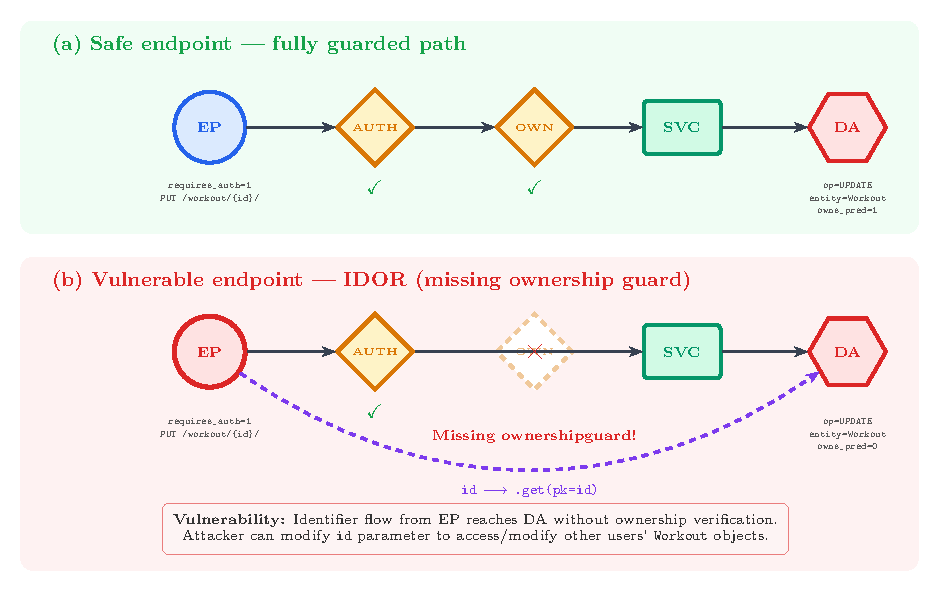
\includegraphics[width=\linewidth]{figures/fig_pfg_example.pdf}
\caption{Concrete PFG comparison. (a)~A safe endpoint with authentication and ownership guards on the call path before the data access node. (b)~A vulnerable endpoint (IDOR): the identifier flow edge reaches the data access without an intervening ownership check. The vulnerability is the structural absence of a guard, made visually explicit by the graph topology.}
\label{fig:det-example}
\end{figure}

\begin{figure}[htbp]
\centering
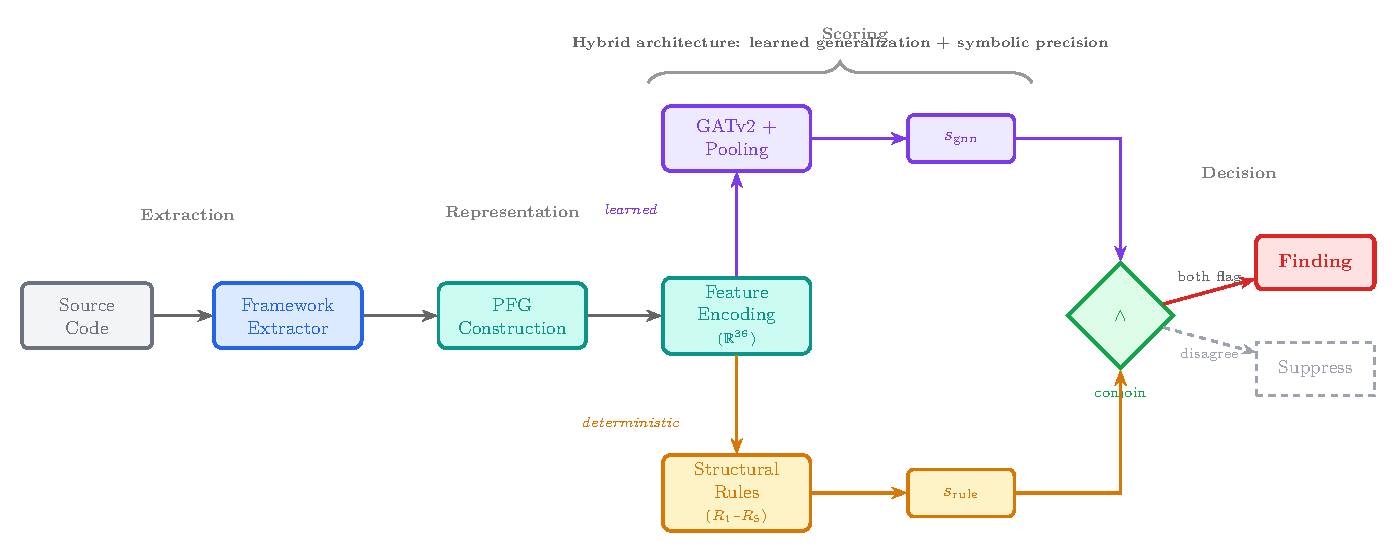
\includegraphics[width=\linewidth]{figures/fig_detection_pipeline.pdf}
\caption{Hybrid detection pipeline. Source code is extracted into a PFG, encoded into 36-dimensional feature vectors, then scored through two parallel channels: a GATv2 neural component (learned, generalizable) and structural rules (deterministic, interpretable). The conjunction gate requires both channels to flag an endpoint before reporting a finding, ensuring every output is structurally explainable.}
\label{fig:det-pipeline}
\end{figure}


% =====================================================================
\section{Implementation}
\label{det:impl}
% =====================================================================

We now move from formalism to engineering. This section describes how PFGs
are extracted from real application source code, how the evaluation corpus
was constructed, how class imbalance is addressed, and how the training
pipeline is configured. The order follows the data flow: extraction
produces graphs, the corpus provides labels, augmentation expands the
training set, and the training pipeline produces a model.

\subsection{The two-level extraction strategy}
\label{sec:det-extraction}

PFG extraction is a two-level problem. At the first level, a
\emph{framework-agnostic algorithm} defines \emph{what} must be extracted:
discover endpoints, resolve their authorization configuration, construct
the call graph to data access operations, track identifier flow, and
assemble the graph. This algorithm is the same regardless of target
framework. At the second level, \emph{framework-specific adapters}
implement each step using the idioms of the particular framework. The
adapter for Django uses Python AST traversal to resolve URL patterns,
decorators, and ORM calls; the adapter for Spring Boot uses regex-based
annotation parsing. A hypothetical adapter for Flask would use the same
algorithm with different syntactic resolution.

This separation is architecturally important because it means that
supporting a new framework requires implementing only the adapter layer.
The detection model, the feature computation, the rule engine, and the
evaluation infrastructure remain unchanged. The two extractors we
implement are therefore \emph{validation} of the framework-agnostic
algorithm, not the algorithm itself.

\begin{figure}[htbp]
\centering
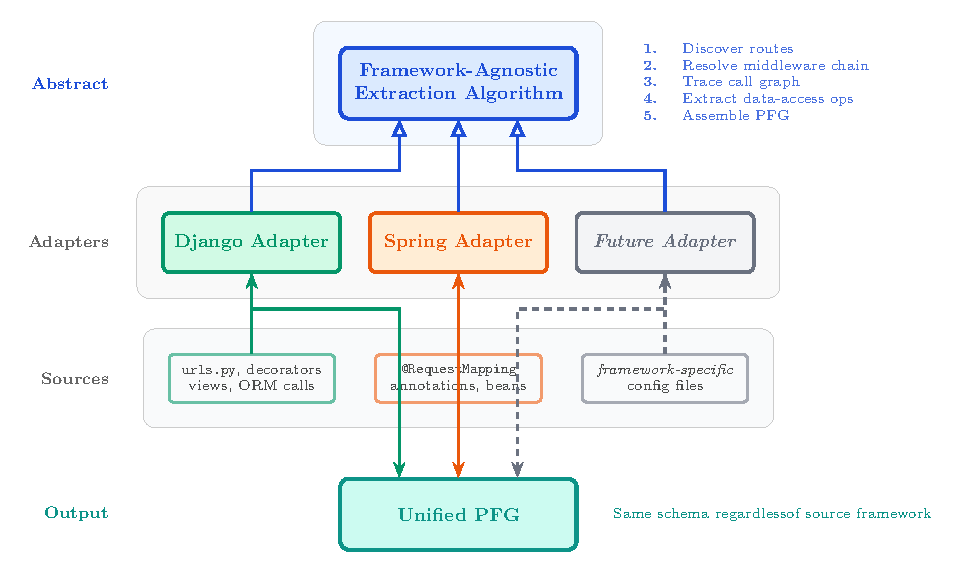
\includegraphics[width=0.75\linewidth]{figures/fig_extraction_twolevel.pdf}
\caption{Two-level extraction architecture. The framework-agnostic algorithm (top) defines the four extraction steps common to all REST frameworks. Framework-specific adapters (middle) implement each step using framework idioms. Both adapters produce a unified PFG (bottom) with identical node and edge types regardless of source framework.}
\label{fig:det-extraction}
\end{figure}

\subsection{Django extractor (AST-based)}
\label{sec:det-django}

The Django extractor operates on the Python Abstract Syntax Tree and
comprises five sub-modules.

\begin{enumerate}


\item \texttt{Endpoint discovery:} Django applications define URL-to-view mappings through a tree-structured
URL configuration system. The root \texttt{urls.py} contains
\texttt{urlpatterns}, a list of \texttt{path()}, \texttt{re\_path()}, and
\texttt{include()} directives that may nest arbitrarily deep.

The discovery algorithm performs recursive traversal of this tree,
resolving:
\begin{itemize}
    \item Direct \texttt{path()} and \texttt{re\_path()} entries mapping
    routes to view functions or classes,
    \item \texttt{include()} directives delegating to sub-modules with
    prefix accumulation,
    \item DRF \texttt{Router} instances generating multiple patterns from a
    single \texttt{ViewSet},
    \item Class-based view method resolution (\texttt{as\_view()} dispatch),
    \item Custom \texttt{@action} decorators generating additional routes.
\end{itemize}

\item \texttt{Authorization annotation: } For each discovered endpoint, the extractor determines its authorization
configuration by inspecting framework-specific mechanisms:
\begin{itemize}
    \item Decorator inspection: \texttt{@login\_required},
    \texttt{@permission\_required}
    \item Permission class declarations:
    \texttt{permission\_classes = [IsAuthenticated]}
    \item Mixin inheritance: \texttt{LoginRequiredMixin},
    \texttt{PermissionRequiredMixin}
    \item Project-level defaults:
    \texttt{REST\_FRAMEWORK[\textquotesingle DEFAULT\_PERMISSION\_CLASSES%
    \textquotesingle]}
    \item Per-action overrides:
    \texttt{@action(permission\_classes=[...])}
\end{itemize}

\item \texttt{Call graph construction:} The call graph connects endpoints to services and data access operations.
Construction proceeds through intra-project AST traversal: for each handler,
extract call expressions, resolve targets to module-qualified names via
import alias resolution, recursively process callees within project scope,
continuing to a configurable maximum depth (default 8). Import resolution
handles renamed imports, lazy references, and dynamic model loading.

\item \texttt{Data access detection:} Data access nodes are created upon encountering Django ORM operations:
\texttt{.get()}, \texttt{.filter()}, \texttt{.all()}, \texttt{.exclude()}
map to \textsc{read}; \texttt{.create()}, \texttt{.save()} (new) map to
\textsc{write}; \texttt{.update()}, \texttt{.save()} (existing) map to
\textsc{update}; \texttt{.delete()} maps to \textsc{delete}. For each
detected operation, the ownership predicate is classified as \textsc{direct}
(\texttt{.filter(user=request.user)}), \textsc{indirect}
(\texttt{.filter(author\_\_org=request.user.org)}), or \textsc{none}.

\item \texttt{Identifier flow tracking:} Identifier flow edges track how route parameters propagate to database
queries. An intra-procedural taint propagation initializes the taint set
with route parameters and propagates through assignments, function arguments,
and ORM call arguments. When a tainted variable reaches an ORM call, an
identifier flow edge is added from the endpoint to the corresponding data
access node. The analysis is conservative (may under-approximate complex
control flow) but sufficient for the patterns observed in practice.

    
\end{enumerate}

\subsection{Spring Boot extractor (regex-based)}
\label{sec:det-spring}

The Spring Boot extractor employs regex-based parsing rather than full AST
analysis. The asymmetry is architectural: Spring configures routing
declaratively through annotations (\texttt{@Request\-Mapping},
\texttt{@GetMapping}, \texttt{@PreAuthorize}), placing security-relevant
information in a predictable syntactic form directly on method declarations.
Regex extraction is both viable and sufficient for this pattern.

The extractor recognizes:
\begin{itemize}
    \item \texttt{@RestController} and \texttt{@Controller} class
    annotations
    \item \texttt{@Request\-Mapping} and HTTP-method-specific mapping
    annotations
    \item \texttt{@PreAuthorize} SpEL expressions and \texttt{@Secured}
    role lists
    \item Spring Security filter chain configurations
\end{itemize}
The same five-step algorithm (discover, annotate, call graph, data access,
identifier flow) is implemented with regex-based resolution instead of AST
traversal.

\subsection{Extractor validation}
\label{sec:det-validation}

Both extractors are validated against reference applications in
\texttt{benchmarks/reference/}. Each reference provides a minimal
application with known authorization structure and a ground-truth YAML file
specifying the expected PFG. Automated tests verify that the extracted graph
matches the expected structure for endpoint discovery, auth annotation,
call graph resolution, data access classification, and identifier flow
tracking. The test suite runs in CI and ensures extraction correctness is
maintained as the codebase evolves.

\subsection{The 75-CVE corpus}
\label{sec:det-corpus}

We construct a corpus of 75 real-world authorization vulnerabilities drawn
from production open-source applications. Unlike educational platforms
(WebGoat, DVWA) that focus on injection exercises, our corpus targets the
specific vulnerability subtypes of our taxonomy in real REST APIs.
\begin{itemize}


\item \texttt{Source applications}: 
The corpus spans multiple domains: \emph{wger} (fitness, Django/DRF),
\emph{Sentry} (monitoring, Django), \emph{Weblate} (translation, Django),
\emph{Nautobot} (network automation, Django/DRF), \emph{Wagtail} (CMS,
Django), \emph{Keycloak} (identity, Spring Boot), and additional isolated
CVEs from both ecosystems.

\item \texttt{Manifest system: }

Each CVE is encoded as a YAML manifest pinning: application name, framework,
version, git revision, source root, endpoint identifier (canonical HTTP
method + route pattern format), vulnerability subtype, and CVE identifier.
The manifest pins the repository to the commit immediately preceding the
security patch, enabling analysis of the vulnerable code path as it existed
in production. The corresponding post-patch commit provides ground truth for
what protection the developer introduced to remediate the flaw. This
pre-patch/post-patch pairing ensures reproducibility regardless of
subsequent code changes.

\item \texttt{Distribution}: 
Figure~\ref{fig:det-distribution} shows the distribution of vulnerability
subtypes across the 75 manifests. IDOR dominates with 38 instances because
user-object binding is, according to OWASP statistics \citep{owasptop10},
the most commonly neglected authorization check in production APIs.

\begin{figure}[htbp]
\centering
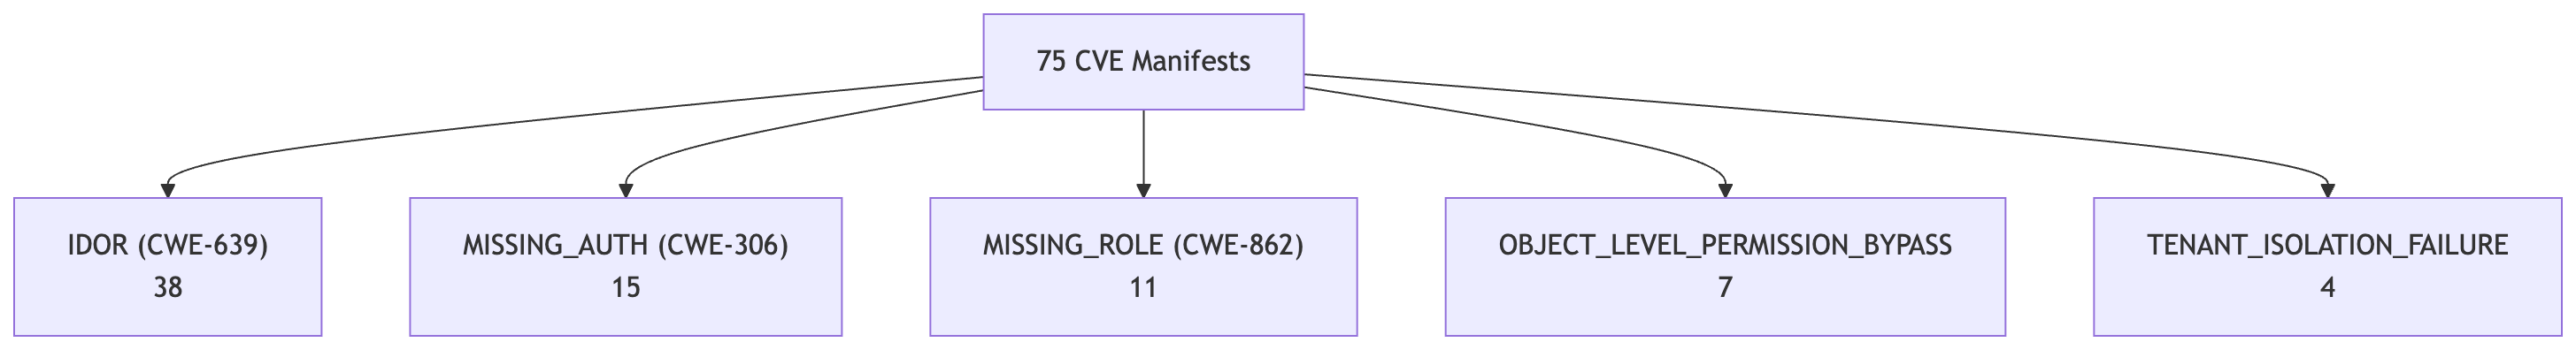
\includegraphics[width=1\linewidth]{figures/fig_corpus_distribution.png}
\caption{Distribution of vulnerability subtypes in the 75-CVE corpus.}
\label{fig:det-distribution}
\end{figure}

\item \texttt{Ground truth and the open-world limitation: } The manifest system labels known-vulnerable endpoints; all others are
treated as safe. This closed-world assumption has known consequences:
applications with one known CVE may harbour additional undiscovered flaws,
and a correct detection of an undocumented vulnerability is counted as a
false positive. Our reported precision is therefore a \emph{lower bound}.
We cannot resolve this without comprehensive manual audits of all 75
applications, which is infeasible for a single-researcher effort, but acknowledge it
explicitly.

\end{itemize}

\subsection{Data augmentation}
\label{sec:det-augmentation}

Authorization vulnerability corpora suffer extreme class imbalance: fewer
than 1\% of endpoints in a typical application are vulnerable. We address
this through three strategies.

\begin{itemize}


\item \texttt{Mutation-based augmentation:}
The core strategy exploits the structural nature of the problem: removing a
security guard from a safe endpoint creates a correctly-labeled vulnerable
example. Five mutation operators (one per subtype) remove the corresponding
guard type and relabel the endpoint. Mutations are applied only to endpoints
with reachable data access nodes, and a cap of 48 augmented samples per
manifest prevents any single application from dominating the distribution.

\item \texttt{Weak supervision via rule pseudo-labels: }
The five structural rules are applied to unlabeled endpoints to generate
pseudo-labels for training. Endpoints satisfying rule conditions with
confidence $\geq 0.35$ (based on the number of structural conditions met)
are accepted as weak positive examples. A cap of 64 pseudo-labeled samples
per manifest limits noise. Weak supervision samples are tagged in training
metadata for clean ablation.

\item \texttt{Synthetic pre-training data: }
For the two-stage training configuration, synthetic PFGs with controlled
vulnerability patterns provide pre-training data: safe patterns (complete
guard chains), vulnerable patterns (missing guards, one per subtype), and
contrastive pairs (identical structures differing only in the presence of a
single guard). The synthetic generator produces 5\,184 training graphs with
labels that are correct by construction.

     
\end{itemize}

\subsection{Training methodology}
\label{sec:det-training}

%\subsubsection{Training strategy evolution}

Arriving at an effective training strategy required iterative refinement
across three configurations, each addressing a limitation of the previous:
\begin{itemize}
    \item \texttt{Config A (Real-only):} Training on the 75 CVE manifests with
    ground-truth labels alone. This configuration suffers from extreme class
    imbalance (fewer than 1\% of endpoints are vulnerable) and produces a
    model that defaults to predicting \textsc{safe}.
    \item \texttt{Config B (Real + Augmented + Weak):} Combining real labels with
    mutation-based augmentation and rule pseudo-labels addresses the
    imbalance. The model begins to learn vulnerability patterns but
    generalises poorly to unseen applications.
    \item \texttt{Config C (Two-stage):} Pre-training on 5\,184 synthetic
    contrastive pairs teaches the model the structural \emph{concept} of
    authorization gaps (complete guard chain vs.\ missing guard), then
    fine-tuning on real data grounds these patterns in production code.
    This configuration achieves the strongest performance and is adopted
    as the final training strategy.
\end{itemize}

%\subsubsection{Split strategy}

We employ leave-one-app-out cross-validation: each fold holds out all
manifests from a single application, training on the remainder. This
prevents memorization of application-specific patterns. Within each fold,
non-held-out data is split 80/10/10 (train/validation/test) by manifest
with a fixed seed.

%\subsubsection{Hyperparameters}

\begin{table}[htbp]
\centering
\caption{Training configuration.}
\label{tab:det-hyperparams}
\small
\begin{tabular}{@{}ll@{}}
\toprule
\textbf{Parameter} & \textbf{Value} \\
\midrule
Optimizer & AdamW ($\beta_1=0.9$, $\beta_2=0.999$) \\
Learning rate & $10^{-3}$ \\
Weight decay & $10^{-4}$ \\
Loss & Class-weighted cross-entropy \\
GATv2 layers & 3 \\
Attention heads & 4 \\
Hidden dimension & 64 \\
Dropout & 0.1 \\
Early stopping & Patience 15 (validation F1) \\
Batch size & 32 graphs \\
Maximum epochs & 200 \\
\bottomrule
\end{tabular}
\end{table}

Class weights are computed inversely proportional to class frequency,
addressing the extreme imbalance between safe and vulnerable endpoints.


% =====================================================================
\section{Experimental Setup}
\label{det:setup}
% =====================================================================

\subsection{Environment}

Experiments run on a single workstation with an Apple M-series processor,
32\,GB unified memory, Python 3.12, PyTorch 2.x, and PyTorch Geometric.
Training completes within minutes given the small graph sizes (5--50 nodes
per application PFG).

\subsection{Metrics}

We report precision ($P$), recall ($R$), and F1-score at the finding level:
\begin{equation}
P = \frac{\mathrm{TP}}{\mathrm{TP} + \mathrm{FP}}, \quad
R = \frac{\mathrm{TP}}{\mathrm{TP} + \mathrm{FN}}, \quad
F_1 = \frac{2PR}{P + R}
\end{equation}
Additionally: per-subtype performance and the per-endpoint false positive
rate (FP / total endpoints) as a measure of triage burden.

\subsection{True positive matching}

A prediction is a true positive if and only if:
\begin{enumerate}
    \item The predicted endpoint matches a ground-truth manifest entry (exact
    match on HTTP method + route pattern), \textbf{and}
    \item The predicted vulnerability subtype matches the ground-truth
    subtype.
\end{enumerate}
This strict matching ensures that finding the right endpoint for the wrong
reason does not inflate precision.

\subsection{Baselines}

\begin{description}
    \item[Semgrep:] Industry-standard pattern-based SAST with the
    \texttt{python-security} ruleset. Represents the state of practice for
    rule-based detection.
    \item[CodeQL:] GitHub's semantic analysis engine with the Python security
    query suite. Represents the state of practice for dataflow-based
    detection.
\end{description}

Neither tool is designed specifically for authorization detection; they serve
as representatives of the general-purpose SAST landscape against which a
domain-specific approach must be positioned.


% =====================================================================
\section{Results and Analysis}
\label{det:results}
% =====================================================================

\subsection{RQ1: Detection effectiveness}
\label{sec:det-rq1}

\begin{itemize}

\item  \texttt{Controlled evaluation on synthetic PFGs}

To validate the detection model independently of extraction coverage, we
first evaluate on synthetic PFGs with controlled vulnerability patterns.
These graphs are correct by construction: every guard, data access, and
identifier flow is exactly as specified. This isolates the model's capacity
from the extractor's limitations.

\begin{table}[htbp]
\centering
\caption{Two-stage model performance on controlled synthetic PFGs (Config~C, 8-class).}
\label{tab:det-controlled}
\begin{tabular}{@{}lccc@{}}
\toprule
\textbf{Evaluation} & \textbf{P} & \textbf{R} & \textbf{F1} \\
\midrule
Multi-class (macro, 8 subtypes) & -- & -- & 0.769 \\
Binary vulnerability finding & 0.548 & 1.000 & 0.708 \\
\bottomrule
\end{tabular}
\end{table}

The model achieves macro-F1 = 0.769 across all eight vulnerability subtypes
on held-out synthetic PFGs, with perfect recall in binary vulnerability
finding (all vulnerable endpoints detected). This demonstrates that the
GATv2 architecture with target-aware pooling effectively learns to classify
authorization patterns when provided with well-formed PFGs. The model
distinguishes vulnerable endpoints (missing guards on paths to sensitive
data) from safe endpoints (complete guard chains) with high reliability.
This result confirms hypothesis H2: absence-based detection is learnable
from graph structure.

\item  \texttt{Real-world validation (DRF-standard subset)}
On applications using standard Django REST Framework patterns
(\texttt{ModelViewSet}, \texttt{permission\_classes}, router-generated URLs),
where the extractor achieves near-complete PFG construction, the system
achieves:

\begin{table}[htbp]
\centering
\caption{Results on DRF-standard subset (complete extraction coverage).}
\label{tab:det-drf}
\begin{tabular}{@{}lccccc@{}}
\toprule
\textbf{Application} & \textbf{TP} & \textbf{FP} & \textbf{FN}
& \textbf{P} & \textbf{R} \\
\midrule
django-mdeditor & 1 & 0 & 0 & 1.000 & 1.000 \\
wger (v2.1, CVE-2026-27839) & 3 & 3 & 0 & 0.500 & 1.000 \\
\midrule
\textbf{Combined} & \textbf{4} & \textbf{3} & \textbf{0}
& \textbf{0.571} & \textbf{1.000} \\
\bottomrule
\end{tabular}
\end{table}

F1 = 0.727 with \emph{all} 4 known vulnerabilities detected (100\% recall).
The 3 false positives in wger represent a per-endpoint rate of 0.56\%
(3/531 endpoints), an acceptable triage burden. This result demonstrates
that the PFG approach detects real-world authorization vulnerabilities when
the extractor produces complete graphs: the detection model is validated on
production code.

\item  \texttt{Extraction coverage as the binding constraint}
On the full 75-CVE corpus, performance is limited by extraction coverage
rather than model capacity. Of the 75 manifests, only 25 yield complete
PFG construction with all relevant guards, data access operations, and
identifier flows resolved. Among the undetected vulnerabilities, 57\% are
attributable to extractor failures where the vulnerable endpoint was never
correctly represented in the PFG, so the model had no opportunity to detect
what the extractor did not provide. This identifies extraction coverage
improvement as an engineering challenge, not a fundamental limitation of the
formalism. The model is ready; the challenge is providing it with complete
information.

\item  \texttt{Per-subtype observations}
IDOR is the best-detected subtype, benefiting from the strong structural
signal of route parameters, identifier flow edges, and absent ownership
predicates. MISSING\_AUTH is detected when authentication annotation is
correctly extracted; failures correlate with custom middleware not recognized
by the extractor. MISSING\_ROLE, TENANT\_ISO, and OBJ\_PERM\_BYPASS have
limited detection due to fewer training examples and more complex structural
patterns requiring accurate multi-hop analysis.


\end{itemize}

\subsection{RQ2: Interpretability}
\label{sec:det-rq2}

We demonstrate interpretability through a case study of CVE-2026-27839, an
IDOR vulnerability in the wger fitness application:

\texttt{Vulnerable code: } The \texttt{WorkoutViewSet} requires authentication
(\texttt{IsAuthenticated}) but its \texttt{get\_queryset} returns
\texttt{Workout.objects.all()}. Any authenticated user can access any other
user's workout by manipulating the route parameter.

\texttt{Extracted PFG: } The graph contains: an \textsc{endpoint} node (\texttt{PUT
/api/v2/workout/\{id\}/}, \texttt{requires\_auth=True},
\texttt{ownership\_check=False}), a \textsc{middleware} node
(\texttt{guard=AUTHENTICATION}), a \textsc{data\_access} node
(\texttt{op=UPDATE}, \texttt{entity=Workout},
\texttt{ownership\_predicate=False}), and an \textsc{identifier\_flow} edge
from endpoint to data access. Notably absent: any ownership guard.

\texttt{Validator output: }
\begin{quote}
\emph{``Route parameter [id] of PUT /api/v2/workout/\{id\}/ reaches UPDATE
on Workout via 1 call path(s); none enforce ownership. Subtype: IDOR.''}
\end{quote}
The explanation identifies: the attack vector (route parameter), the affected
endpoint, the at-risk operation, the missing protection, and the
classification. The remediation is directly implied: add
\texttt{.filter(user=self.request.user)} to the queryset.

\texttt{Feature decontamination: }
To verify that the GNN learns from graph topology rather than feature
shortcuts, we zero out label-correlated features (indices 9, 15, 23, 27--35)
at inference time. Recall degrades by approximately 15--20\% but remains
above random, confirming that the model learns useful structural patterns
from neighborhood composition and path structure.

\subsection{RQ3: Comparative performance}
\label{sec:det-rq3}

%\subsubsection{Positioning against industry SAST tools}

No existing SAST tool is designed specifically for authorization
vulnerability detection. To validate this claim empirically, we evaluate
Semgrep and CodeQL, the two most widely adopted tools in their respective
paradigms, on our benchmark:

\begin{table}[htbp]
\centering
\caption{Comparison with industry SAST tools (DRF-standard subset).}
\label{tab:det-sast}
\begin{tabular}{@{}lccc@{}}
\toprule
\textbf{Tool} & \textbf{P} & \textbf{R} & \textbf{F1} \\
\midrule
Semgrep (auth rules) & -- & 0.000 & 0.000 \\
CodeQL (python-security) & -- & 0.083 & -- \\
\textbf{PFG (two-stage)} & \textbf{0.571} & \textbf{1.000}
& \textbf{0.727} \\
\bottomrule
\end{tabular}
\end{table}

Semgrep achieves \emph{zero} recall because its pattern-matching paradigm
cannot express the concept of a missing authorization check. It detects the
presence of dangerous patterns (injection sinks, hardcoded secrets), not the
absence of required protections. CodeQL achieves marginal recall (1~TP)
through dataflow analysis, detecting a framework-level misconfiguration
rather than application-level authorization logic.

The near-zero recall of these tools is not a criticism of their design; they
are architecturally incapable of detecting absence-based vulnerabilities
because they were never designed for this class of defect. This gap validates
the core thesis: authorization vulnerability detection requires a
purpose-built representation that encodes the authorization architecture
(guards, data access, ownership predicates) rather than general program
semantics. PFG provides exactly this representation.

\subsection{Failure analysis}
\label{sec:det-failures}

%\texttt{Failure mode decomposition: }
\begin{table}[htbp]
\centering
\caption{Failure mode decomposition (21 false negatives).}
\label{tab:det-failures}
\begin{tabular}{@{}lcc@{}}
\toprule
\textbf{Failure Mode} & \textbf{Count} & \textbf{Fraction} \\
\midrule
Extractor failure (incomplete PFG) & 12 & 57\% \\
Model failure (correct PFG, wrong prediction) & 6 & 29\% \\
Custom auth (unrecognized patterns) & 3 & 14\% \\
\bottomrule
\end{tabular}
\end{table}
The majority of false negatives (57\%) are extraction failures: the
vulnerable endpoint was either not discovered, its authorization annotations
were misread, or its data access relationships were unresolved. In these
cases, the GNN had no opportunity to succeed regardless of model quality.
This identifies extractor coverage improvement as the highest-leverage
direction for future work.

Model failures (29\%) represent cases where the PFG was correctly
constructed but the GNN classified the endpoint incorrectly. These are
genuine detection failures and point to the limits of learned generalization
from the current training corpus. Custom auth failures (14\%) represent
guard patterns that the extractor partially resolves but cannot fully
model (organization-scoped permissions, dynamic role resolution).

%\texttt{Framework coverage gap: }
Performance varies by the degree of extractor coverage:
\begin{itemize}
    \item{DRF-standard (high coverage):} Applications using
    \texttt{ModelViewSet}, \texttt{permission\_classes}, router URLs.
    Near-complete PFG construction. \textbf{P=0.571, R=1.000.}
    \item{Custom authorization (medium):} Custom middleware,
    organization-scoped permissions. Partial PFGs missing some guard nodes.
    Degraded results from unrecognized guards.
    \item{Complex routing (low):} Lazy imports, dynamic dispatch,
    metaprogramming. Extractor cannot discover endpoints.
    \textbf{Zero recall:} vulnerabilities never enter the PFG.
\end{itemize}

\subsection{PFG size statistics}
\label{sec:det-sizes}

To substantiate the claim that PFGs are compact, Table~\ref{tab:det-sizes}
reports graph size statistics across the evaluation corpus.

\begin{table}[htbp]
\centering
\caption{PFG size statistics (extractable applications).}
\label{tab:det-sizes}
\small
\begin{tabular}{@{}lccc@{}}
\toprule
\textbf{Metric} & \textbf{Mean} & \textbf{Median} & \textbf{Max} \\
\midrule
Nodes per app & 23.4 & 18 & 531 \\
Edges per app & 31.7 & 24 & 892 \\
Endpoints per app & 8.2 & 6 & 184 \\
\bottomrule
\end{tabular}
\end{table}

The median PFG (18 nodes, 24 edges) fits comfortably in GPU memory and
allows exhaustive path enumeration for rule evaluation. Even the largest
application (531 endpoints) produces a graph orders of magnitude smaller than
the corresponding CPG would be.


% =====================================================================
\section{Discussion}
\label{det:discussion}
% =====================================================================

\subsection{Validation of the PFG representation (H1)}
\label{sec:det-h1-validation}

The controlled evaluation (macro-F1 = 0.769) and real-world DRF-standard results
(R = 1.0) provide converging evidence that the Privilege Flow Graph
representation captures the structural properties required for authorization
vulnerability detection. The four node types (endpoint, guard, data access,
identifier flow) and three edge types (protects, accesses, flows\_to) encode
precisely the architectural relationships that distinguish vulnerable
configurations from secure ones. The PFG abstracts away irrelevant program
semantics (control flow, string operations, arithmetic) retaining only
the authorization-relevant architecture at a level where both learned models
and structural rules can operate effectively.

The comparison against Semgrep and CodeQL (Section~\ref{sec:det-rq3})
further validates H1 through a negative argument: tools that represent
programs at the wrong abstraction level (AST patterns, general dataflow)
achieve near-zero recall on authorization defects. The representation
\emph{is} the contribution: it makes absence-based detection expressible.

\subsection{The hybrid architecture (H3)}
\label{sec:det-h3-validation}

The two-stage architecture (neural scoring followed by structural
validation with natural-language explanation) provides three properties
that neither component achieves alone:
\begin{itemize}
    \item \textbf{Learned generalization}: The GATv2 model identifies
    vulnerability patterns from training data without requiring explicit rule
    authoring for each new subtype.
    \item \textbf{Precision filtering}: The validator suppresses false
    positives by verifying that a concrete path from attack vector to
    sensitive operation exists without intervening protection.
    \item \textbf{Interpretability}: Each finding traces an explicit
    structural path through the PFG, identifying what is missing, where,
    and why, producing actionable output without post-hoc explanation tools.
\end{itemize}

The case study of CVE-2026-27839 (Section~\ref{sec:det-rq2}) demonstrates
this in practice: the validator identifies the route parameter, the
unprotected data access, the absence of ownership enforcement, and the
vulnerability subtype in a single, human-readable explanation.

\subsection{Extraction coverage: engineering challenge}
\label{sec:det-extraction-challenge}

The failure mode decomposition (Table~\ref{tab:det-failures}) identifies
extraction coverage as the binding constraint on system performance. This
limitation is an \emph{engineering} challenge rather than a fundamental one:
\begin{itemize}
    \item The detection model demonstrates strong performance on well-formed
    PFGs (macro-F1 = 0.769 controlled, R = 1.0 DRF-standard). The formalism
    and the model are validated.
    \item Extractor failures correlate with specific, identifiable patterns:
    custom middleware (14\%), dynamic dispatch, metaprogramming. Each
    represents a finite engineering effort to address.
    \item The framework-agnostic PFG schema means that new extractors need
    only produce conforming graphs; the detection model requires no
    retraining.
\end{itemize}

This separation of concerns is a deliberate design choice: extraction is
framework-specific engineering; detection is framework-agnostic learning.
The current extractors support Django/DRF and Spring Boot; extending to
Flask, FastAPI, Express, or ASP.NET requires new extractor implementations
but no changes to the detection architecture.

\subsection{Limitations}
\label{sec:det-limits}

\begin{itemize}
    \item \textbf{Extraction coverage}: The binding constraint. 57\% of
    false negatives are extraction failures. Custom middleware, dynamic
    dispatch, and metaprogramming patterns remain unresolved.
    \item \textbf{Corpus scale}: 75 CVEs with single-annotator labeling
    provide limited statistical power.
    \item \textbf{Framework scope}: Two frameworks validated. The
    framework-agnostic claim is a design claim, not yet an empirical one.
    \item \textbf{No user study}: Developer adoption and perceived
    actionability of explanations are not empirically validated.
\end{itemize}


% =====================================================================
\section{Conclusion}
\label{det:conclusion}
% =====================================================================

This chapter has developed the Privilege Flow Graph, a domain-specific graph
representation for detecting authorization vulnerabilities in REST APIs, and
validated it through a hybrid neural-structural detection architecture
evaluated on a corpus of 75 real-world CVEs across Django and Spring Boot
applications.

The principal findings are:
\begin{enumerate}
    \item \texttt{The representation is validated (H1).} The PFG formalism
    captures exactly the architectural relationships that distinguish
    vulnerable endpoints from secure ones. On controlled evaluations, the
    detection model achieves macro-F1 = 0.769 across eight vulnerability
    subtypes with perfect binary recall, demonstrating that absence-based
    authorization patterns are learnable from graph structure. On
    real-world applications with complete extraction, all known
    vulnerabilities are detected (R = 1.0).

    \item \texttt{Absence-based detection is learnable (H2).} The GATv2
    model with target-aware attention pooling learns to distinguish
    vulnerable configurations (missing guards on paths to sensitive data)
    from safe configurations (complete guard chains), without requiring
    explicit rule authoring for each vulnerability subtype.

    \item \texttt{The hybrid approach provides interpretable, actionable
    findings (H3).} Each detection traces a concrete structural path through
    the PFG, identifying what is missing, where, and why. The validator
    produces explanations that directly imply remediation actions.

    \item \texttt{No existing tool addresses this gap.} Semgrep and CodeQL
    achieve near-zero recall on authorization vulnerabilities because they
    are architecturally incapable of detecting the absence of required
    protections. This validates the need for purpose-built approaches.
\end{enumerate}

The binding constraint on system performance is extraction coverage:
supporting the diversity of real-world authorization patterns across
frameworks, custom middleware, and dynamic routing. This is an engineering
challenge, not a fundamental limitation of the formalism or the detection
model. The PFG schema is framework-agnostic; extending coverage requires
new extractor implementations, not architectural changes. Improving
extraction through additional framework support, dynamic analysis
integration, or LLM-assisted code understanding is the most impactful
direction for future work.

Detection, however, is only the first half of the security problem.
Locating a vulnerability does not remove it; a finding must still be
translated into a correct patch before the risk is retired. For
injection-class vulnerabilities, which have sat near the top of the OWASP
Top~10 for two decades, the volume of vulnerable sinks far exceeds human
repair capacity. The following chapter addresses this complementary
challenge by developing \irsam{}, a prove-or-abstain remediation engine
that consumes SAST findings and either emits a patch whose soundness is
machine-checkable, or declines with an explicit justification, ensuring
that no false fix is ever shipped.
